\documentclass[11pt,landscape,a4paper,fleqn]{article}
\usepackage[utf8]{inputenc}
\usepackage[ngerman]{babel}
\usepackage{tikz}
\usepackage{bbm}
\usetikzlibrary{shapes,positioning,arrows,fit,calc,graphs,graphs.standard}
\usepackage[nosf]{kpfonts}
\usepackage[t1]{sourcesanspro}
%\usepackage[lf]{MyriadPro}
%\usepackage[lf,minionint]{MinionPro}
\usepackage{multicol}
\usepackage{wrapfig}
\usepackage[top=5mm,bottom=5mm,left=5mm,right=5mm]{geometry}
\usepackage[framemethod=tikz]{mdframed}
\usepackage{microtype}
\usepackage{paralist} % for compacter lists
\usepackage{bm}
\usepackage{algorithm}
\usepackage{algpseudocode}
\usepackage{comment}
\usepackage{amsmath}
\usepackage{dsfont}

\makeatletter
\def\BState{\State\hskip-\ALG@thistlm}
\makeatother


\let\bar\overline

\definecolor{myblue}{cmyk}{1,.72,0,.38}
\definecolor{myorange}{cmyk}{0,0.7,0.8,0}
\definecolor{myred}{cmyk}{0,1,0.75,0}

\pgfdeclarelayer{background}
\pgfsetlayers{background,main}

\everymath\expandafter{\the\everymath \color{myblue}}
%\everydisplay\expandafter{\the\everydisplay \color{myblue}}

\renewcommand{\baselinestretch}{.8}
\pagestyle{empty}

\global\mdfdefinestyle{header}{%
linecolor=gray,linewidth=1pt,%
leftmargin=0mm,rightmargin=0mm,skipbelow=0mm,skipabove=0mm,
}

\makeatletter
\renewcommand{\section}{\@startsection{section}{1}{0mm}%
                                {.2ex}%
                                {.2ex}%x
	                                {\color{myred}\sffamily\small\bfseries}}
\renewcommand{\subsection}{\@startsection{subsection}{1}{0mm}%
                                {.2ex}%
                                {.2ex}%x
                                {\color{myorange}\sffamily\bfseries}}
\renewcommand{\subsubsection}{\@startsection{subsubsection}{1}{0mm}%
	{.2ex}%
	{.2ex}%x
	{\sffamily\bfseries}}


% math helpers
\DeclareMathOperator*{\argmin}{arg\,min}
\DeclareMathOperator*{\argmax}{arg\,max}
\newcommand{\E}{\mathbb{E}}

\makeatother
\setlength{\parindent}{0pt}

\newcommand{\imp}[1]{\boxed{\boldsymbol{#1}}} % Einrahmung und Fett
\newcommand{\w}{\omega}
\newcommand{\ud}{\,\mathrm{d}}% Differential
\newcommand{\norm}[1]{\left\lVert#1\right\rVert}
\newcommand{\X}{\mathcal{X}}

% compress equations
%\medmuskip=0mu
%\thinmuskip=0mu
%\thickmuskip=0mu

\begin{document}
\small
\begin{multicols*}{4}
	\section{Basics}
$f(x) = \frac{1}{\sqrt{2\pi \sigma^2}} e^{- \frac{1}{2} \frac{(x-\mu)^2}{\sigma^2}},\quad \mathcal{N}(x|\mu, \sigma)$\\
$f(x) = \frac{1}{\sqrt{(2\pi)^d\det\Sigma}} e^{- \frac{1}{2} (x-\mu)^T \Sigma^{-1} (x-\mu)},\quad \mathcal{N}(x|\mu, \Sigma)$\\
Condition number: $\kappa(A)=\frac{\sigma_{max}(A)}{\sigma_{min}(A)}$ \\
f(x) on a: $f(a)+\tfrac{f'(a)}{1!}(x-a) + \tfrac{f''(a)}{2!}(x-a)^2 + ...$ \\
Binomial: $f(k,n,p) {=} Pr(X=k) {=} \binom nk p^k (1{-}p)^{n{-}k}$ \\
$\ln(p(x|\mu, \Sigma)) {=} {-}\tfrac{d}{2}\ln(2\pi) {-} \tfrac{\ln|\Sigma|}{2} {-} \tfrac{1}{2}(x{-}\mu)^T\Sigma(x{-}\mu)$ \\
$X {\sim} \mathcal{N}(\mu,\Sigma)$, $Y{=}A{+}BX \Rightarrow Y{\sim}\mathcal{N}(A{+}B\mu,B\Sigma B^T)$ //
General p-norm: $\norm{ x }_p = (\sum_{i=1}^n |x_i|^p)^{1/p}$

\subsection*{Moments}
\begin{inparaitem}[\color{red}\textbullet]
% Variance
\item $Var[X]=\int_x(x-\mu)^2p(x) dx$ \\
\item $Var[X]=E[(X-E[X])^2]=E[X^2]-E[X]^2$ \\
\item $Var[X{+}Y]=Var[X]{+}Var[Y]{+}2Cov[X,Y]$ \\
% Covariance
\item $Cov[X,Y] = E[(X - E[X])(Y - E[Y])]$ \\
\item $Cov[aX,bY]{=}abCov[X,Y]$ \\
\item $K_{\bm{XY}} = cov(X,Y) = E[XY^T] - E[X]E[Y^T]$
\end{inparaitem}
\subsection*{Calculus}
\begin{inparaitem}[\color{red}\textbullet]
	\item Part.: $\int u(x)v'(x) dx = u(x)v(x) - \int v(x)u'(x) dx$\\
	\item Chain r.: $\frac{f(y)}{g(x)} = \frac{dz}{dx} \Big|_{x=x_0}= \frac{dz}{dy}\Big|_{z=g(x_0)}\cdot \frac{dy}{dx} \Big|_{x=x_0}$ \\
	%\item $g_x(1) = g_x(0) + g'_x(0) + \int_{0}^{1} g_x''(s)(1-s) ds$ \\
	%\item $g(\mathbf{w}+\delta) - g(\mathbf{w}) = %\int_{\mathbf{w}}^{\mathbf{w+\delta}} \nabla g(\mathbf{u}) du = (\int_{0}^{1} \nabla g(\mathbf{w}+t\delta)dt) \cdot \delta$\\
	\item $\frac{\partial}{\partial \mathbf{x}}(\mathbf{b}^\top \mathbf{x}) = \frac{\partial}{\partial \mathbf{x}}(\mathbf{x}^\top \mathbf{b}) = \mathbf{b}$
	\item $\frac{\partial}{\partial \mathbf{x}}(\mathbf{x}^\top \mathbf{x}) = 2\mathbf{x}$ \\
	\item $\frac{\partial}{\partial \mathbf{x}}(\mathbf{x}^\top \mathbf{A}\mathbf{x}) = (\mathbf{A}^\top + \mathbf{A})\mathbf{x} \stackrel{\text{\tiny A sym.}}{=} 2\mathbf{A}\mathbf{x}$ \\
	\item $\frac{\partial}{\partial \mathbf{x}}(\mathbf{b}^\top \mathbf{A}\mathbf{x}) = \mathbf{A}^\top \mathbf{b}$
	\item $\frac{\partial}{\partial \mathbf{X}}(\mathbf{c}^\top \mathbf{X} \mathbf{b}) = \mathbf{c}\mathbf{b}^\top$ \\
	\item $\frac{\partial}{\partial \mathbf{X}}(\mathbf{c}^\top \mathbf{X}^\top \mathbf{b}) = \mathbf{b}\mathbf{c}^\top$
	\item $\frac{\partial}{\partial \mathbf{x}}(\| \mathbf{x}-\mathbf{b} \|_2) = \frac{\mathbf{x}-\mathbf{b}}{\|\mathbf{x}-\mathbf{b}\|_2}$ \\
	\item $\frac{\partial}{\partial \mathbf{x}}(\|\mathbf{x}\|^2_2) = \frac{\partial}{\partial \mathbf{x}} (\|\mathbf{x}^\top \mathbf{x}\|_2) = 2\mathbf{x}$
	\item $\frac{\partial}{\partial \mathbf{X}}(\|\mathbf{X}\|_F^2) = 2\mathbf{X}$ \\
	\item $x^T A x = Tr(x^T A x) = Tr(x x^T A) = Tr(A x x^T)$ \\
	\item $\tfrac{\partial}{\partial A} Tr(AB) {=} B^T$
	\item $\frac{\partial}{\partial A} log|A| {=} A^{-T}$ \\
	\item $\text{sigmoid}(x) = \sigma(x) = \frac{1}{1+\exp(-x)}$ \\
	\item $\nabla \text{sigmoid}(x) = \text{sigmoid}(x)(1-\text{sigmoid}(x))$ \\
	\item $\nabla \text{tanh}(x) = 1-\text{tanh}^2(x)$ 
	\item $tanhx {=} \frac{sinhx}{coshx} {=} \frac{e^{x}-e^{-x}}{e^{x} + e^{x}}$
\end{inparaitem}
\subsection*{Probability / Statistics}
\begin{compactdesc}
	\item[Bayes' Rule]$ P(Y|X) = \frac{P(X|Y)P(Y)}{P(X)}\frac{P(X|Y)P(Y)}{\sum\limits^k_{i=1}P(X|Y_i)P(Y_i)}$\\
	\item[MGF] $\mathbf{M}_X(t)=\mathbb{E}[e^{\mathbf{t}^T \mathbf{X}}]$, $\mathbf{X}=(X_1,.., X_n) $
\end{compactdesc}
\subsection*{Jensen's inequality}
	X:random variable \& $\varphi$:convex function $\rightarrow$ $\varphi(\mathbb{E}[X]) \leq \mathbb{E}[\varphi(X)]$

	% -*- root: Main.tex -*-
\section{Regression}
%\subsection*{Linear Regression}
%Error: $\hat{R}(w) = \sum_{i=1}^n (y_i - w^Tx_i)^2 = ||Xw-y||^2_2$\\
%Closed form: $w^*=(X^T X)^{-1} X^T y$\\
%Gradient: $\nabla_w \hat{R}(w) = 2X^T (Xw-y)$
\subsection*{Estimation}
Consistency: $\hat{\theta_n} \stackrel{\text{\tiny P}}{\rightarrow} \theta$,
i.e. $\forall\epsilon P \{|\hat{\theta_n}-\theta| \geq\epsilon\} \stackrel{\tiny n \to\infty}{\longrightarrow} 0 $\\
Asymptotic normality: $\sqrt{N}(\theta - \hat{\theta_n}) \to \mathcal{N}(0, J^{-1}IJ^{-1})$ \\
Asymptotic efficiency: $\hat{\theta_n}$ has the smallest variance among all possible consistent estimators (for large enough N), i.e. $\lim_{n\to\infty} (V[\hat{\theta_n}]I(\theta))^{-1} = 1$
	$\hat{\theta}_{MAP} := \argmax_\theta \left \{ \sum_{i=1}^n log(p(x_i | \theta) + log(p(\theta)) \right\}$
\subsection*{Rao-Cramer}
$\Lambda = \frac{\partial \log \mathbb{P}(x|\theta )}{\partial \theta}$ (score function), $E[\Lambda ]=0$\\
Fisher information: $I= \mathbb{V}[\Lambda]$ \\
$J= E[\Lambda^{2}]= -E[\frac{\partial^2 \log \mathbb{P}(x|\theta ) }{\partial \theta \partial \theta ^{T}}]= -E[\frac{\partial \Lambda}{\partial \theta}]$ \\
variance of an estimator is bounded from below by the inverse of Fisher information \\
MSE bound: $E[(\hat \theta -\theta )^{2}] \geq \frac{[1 + b^{\prime} (\theta)]^{2}}{n E[\Lambda ^{2}]} + b_{\hat \theta}^{2}$ \\
Biased estimators: $var(\hat{\theta}) \geq \frac{[1 + b^{\prime}(\theta)]^2}{I(\theta)}$ \\
Efficiency: $e(\hat{\theta}) = \frac{I(\theta)^{-1}}{var(\hat{\theta})} \leq 1$ \\
Cauchy-Schwarz: $|E(X,Y)|^2 \leq E(X^2) E(Y^2)$ 

\subsection*{Regularized regression}
Error: $\hat{R}(w) = \sum \limits_{i=1}^n (y_i - w^Tx_i)^2 + \lambda ||w||_2^2$ (Ridge) \\
Closed form: $w^*=(X^T X + \lambda I)^{-1} X^T y$ (Ridge)\\
%Grad: $\nabla_w \hat{R}(w) = -2 \sum_{i=1}^n (y_i-w^T x_i) \cdot x_i + 2 \lambda w$\\
{\small{} Shrinkage:} $Xw^*{=}\sum_{j=1}^{d} u_j\frac{\sigma_j^2}{\sigma_j^2+\lambda}u_j^Ty$, $X{=}U\Sigma V^T$ 
LASSO: $w^* = \underset{w}{\operatorname{argmin}} \sum \limits_{i=1}^n (y_i - w^Tx_i)^2 + \lambda ||w||_1$

\subsection*{Bayesian linear regression}
	Model:  \= $y = X^T \beta + \epsilon$, with $\epsilon \sim
	\mathcal{N}(\epsilon | 0, \sigma^2 I)$ or 
	\> $P(y | X, \beta, \sigma) = \mathcal{N}(y | X^T \beta , \sigma^2 I)$ 
	$P(\beta | \Lambda) = \mathcal{N} (\beta | 0, \Lambda^{-1})$, Post: $P(\beta | X, y, \Lambda) = \mathcal{N}(\beta | \mu_\beta, \Sigma_\beta)$ 
	$\mu_\beta = (X^T X + \sigma^2 \Lambda)^{-1} X^T y$, $\Sigma_\beta = \sigma^2(X^T X + \sigma^2 \Lambda)^{-1}$ 
	Prediction: \> $y_{new} = \hat{\beta}_{\scaleto{MAP}{4pt}}^T x_{new} = \mu_\beta ^T x_{new}$ 
	$P(y_{new} | x_{new}, X, y, \beta) 
	= \mathcal{N}(\mu_\beta ^T x_{new}, \sigma^2 + x_{new}^T \Sigma_\beta x_{new})$

\subsection*{Combination of Regression Models:}
$\text{bias}[\hat{f}(x)] = \frac{1}{B} \sum_{i=1}^{B} \text{bias}[\hat{f}_i(x)]$\\
Var$[\hat{f}(x)] = \frac{1}{B^2}\sum_i$ Var$[\hat{f}_i(x)]
+ \frac{1}{B^2}\sum_{i,j:i\neq j}$ Cov$[\hat{f}_i(x), \hat{f}_j(x)] \approx \frac{\sigma^2}{B}$
% \subsection*{Smoothing Splines}
% $RSS(f,\lambda) = \sum\limits_{i=1}^n (y_i - f(x_i))^2 + \lambda  \int (f''(x))^2dx$\\

\subsection*{RSS Estimator}
$\hat{\beta} \sim \mathcal{N}(\beta,(X^TX)^{-1}\sigma^2)$.
%\textbf{Unbiasedness}: $\mathbb{E}[\hat{\beta}] = \mathbb{E}[(X^TX)^{-1}X^Ty] = (X^TX)^{-1}X^T\mathbb{E}[X\beta+\epsilon] = (X^TX)^{-1}(X^TX)\beta+X^T\mathbb{E}[\epsilon] = \beta + 0$
%\textbf{Variance of} $a^T\hat{\beta}$: $\mathbb{V}(a^T(X^TX)^{-1}X^T(X\beta + \epsilon)) = \mathbb{V}(a^T\beta) + \mathbb{E}(a^T(X^TX)^{-1}X^T\epsilon\epsilon^TX(X^TX)^{-1}a) = \sigma^2 a^T(X^TX)^{-1}a$ 

%\subsection*{Gauss-Markov Theorem}
%For any linear estimator $\widetilde{\theta}=c^T\mathbf{y}$ that is unbiased for $a^T\beta$ it holds: $\mathbb{V}(a^T\hat{\beta}) \leq \mathbb{V}(c^T\mathbf{y})$\\
%Proof: Let $c^T \mathbf{y} = a^T\hat{\beta} + a^T\mathbf{D}\mathbf{y} = a^T((\mathbf{X^TX})^{-1}\mathbf{X}^T + \mathbf{D})\mathbf{y}$ be an unbiased estimator of $a^T \beta$; then it follow $a^T \mathbf{DX}\beta = 0$ which implies $\mathbf{DX} = 0$.\\
%$\mathbb{V}(c^T \mathbf{y}) = \mathbb{E}[(c^T \mathbf{y})^2]-\mathbb{E}(c^T \mathbf{y})^2 = c^T(\mathbb{E}\mathbf{y}\mathbf{y}^T - \mathbb{E}\mathbf{y}\mathbb{E}\mathbf{y}^T)c = \sigma^2 c^T c $
%= $\sigma^2 \big( a^T ((\mathbf{X^T X})^{-1}\mathbf{X}^T + \mathbf{D}) (\mathbf{X}(\mathbf{X^T X})^{-1}+\mathbf{D}^T)a \big )$\\
%= $\sigma^2 \big( a^T (\mathbf{X^T X})^{-1}a +\mathbf{DD^T}a \big )$
%= $\mathbb{V}(a^T\hat{\beta}) + a^T \mathbf{DD^T}a \geq \mathbb{V}(a^T\hat{\beta})$ (note: $\mathbf{DD^T}$ is PSD)

\subsection*{Bias vs. Variance}
\setlength{\mathindent}{0cm}
$
\E_D\E_{X,Y}\left(\hat{f}(X)-Y\right)^2 = \\
\E_D\E_X\left(\hat{f}(X) - \E(Y|X)\right)^2 + \E_{X,Y}\left(Y - \E(Y|X)\right)^2\\
= \E_X \E_D\left(\hat{f}(X) - \E_D(\hat{f}(X))\right)^2 \text{(variance)}\\
+ \E_X\left(\E_D(\hat{f}(X)) - \E(Y|X)\right)^2 \text{(bias}^2)\\
+ \E_{X,Y}\left(Y - \E(Y|X)\right)^2 \text{(noise)}
$\\
%High bias can cause an algorithm to miss the relevant relations between features and target outputs (underfitting).\\
%High variance can cause overfitting: modeling the random noise in the training data, rather than the intended outputs.

% \subsection*{Gradient Descent}
% 1. Start arbitrary $w_o \in \mathbb{R}$\\
% 2. For $i$ do $w_{t+1} = w_t - \eta_t \nabla \hat{R}(w_t)$

%\subsection*{Curse of Dimensionality}
%To obtain a reliable estimate at a given regularity, the required number of samples grows exponentially with the dimension of the sample space.

% \subsection*{Expected Error}
% For generalization, minimize the expected error
% $R(w) = \int P(x,y) (y-w^Tx)^2 \partial x \partial y$\\
% $= \mathbb{E}_{x,y}[(y-w^Tx)^2]$


\subsection*{Ridge Parametric to nonparametric}
Ansatz: $w=\sum_i \alpha_i x$\\
$w^* = \underset{w}{\operatorname{argmin}} \sum_i (w^Tx_i-y_i)^2 + \lambda ||w||_2^2$ = \\
${\operatorname{argmin}}_{\alpha_{1:n}} \sum_{i=1}^n (\sum_{j=1}^n \alpha_j x_j^T x_i - y_i)^2 + \lambda \sum_i \sum_j \alpha_i \alpha_j (x_i^T x_j)$\\
$= {\operatorname{argmin}}_{\alpha_{1:n}} \sum_{i=1}^n (\alpha^T K_i - y_i)^2 + \lambda \alpha^T K \alpha$\\
$= {\operatorname{argmin}}_{\alpha} ||\alpha^T K -y||_2^2 + \lambda \alpha^T K \alpha$\\
Closed form: $\alpha^* = (K+\lambda I)^{-1} y$\\
Prediction: $y^*= w^{*T} x = \sum_{i=1}^n \alpha_i^* k(x_i,x)$

	% -*- root: Main.tex -*-
\section{Gaussian Processes}
% A GP $\{X_t\}_t$ is a collection of random variables from which any finite sample has a joint Gaussian distribution.\\
% For any finite set of points $T=\{t_1, \dots, t_n\}$ from a GP, it hold that $(X_{t_1}, \dots,X_{t_n})\sim \mathcal{N}(\pmb{\mu_T},\pmb{\Sigma_T})$ with $\pmb{\mu_T} = (\mu(t_1),\dots,\mu(t_n))$, $\pmb{\Sigma_T}(i,j)=k(X_{t_i},X_{t_j})$
\subsection*{Gaussian Process}
%$p\big(\begin{bmatrix}
%\mathbf{y} \\
%y^*\\
%\end{bmatrix}|x^*,\mathbf{X}, \sigma \big) = \mathcal{N}\big(\begin{bmatrix}
%\mathbf{y} \\
%y^*\\
%\end{bmatrix} | \mathbf{0},\begin{bmatrix}
%\mathbf{C_n} & \mathbf{k} \\
%\mathbf{k}^T & c 
%\end{bmatrix}  \big)$\\
%with $\mathbf{C_n} = \mathbf{K} + \sigma^2 \mathbf{I}, c = k(x_{n+1},x_{n+1}) + \sigma^2,\\
%\mathbf{k}=k(x_{n+1}, \mathbf{X}), \mathbf{K}=k(\mathbf{X}, \mathbf{X})$\\
%$p(y^*|x^*, X, y) = \mathcal{N}(y^*|\mu, \sigma^2)$\\
%with $\mu = k^T C_n^{-1}y, \sigma^2 = c-k^TC_n^{-1}k$\\

$[y_1, y_2, ...]^T\!=\!X\beta\!+\!\epsilon \sim \mathcal{N}(y|0,X \Lambda^{-1} X^T+ \sigma^2 I) $
$y \sim \mathcal{N}(y | m(X), K(X,X) + \sigma^2 I) = P(y|X,\Theta)$ 

%Joint dist.: {\footnotesize $p([y, y_{n+1}] | x_{n+1}, X, \sigma) 
%\sim \mathcal{N}([y, y_{n+1}]|, K_{n+1} + \sigma^2I)$}
                    
$\left[\begin{smallmatrix} y \\y_{n+1}\end{smallmatrix}\right] \sim \mathcal{N}\left(\left[\begin{smallmatrix} y \\y_{n+1}\end{smallmatrix}\right]|[\begin{smallmatrix} m(X) \\m(x_{n+1})\end{smallmatrix}], [\begin{smallmatrix} C_n & k \\ k^T & c\end{smallmatrix}]\right)$
	
$p(y_{n+1}|x_{n+1}, X, y)) = \mathcal{N}(y_{n+1} | \mu_{n+1}, \sigma^2_{n+1})$	\\
$\mu_{n+1} = m(x_{n+1})+k^T C^{-1}_n (y\!-\!m(X))$ \\
$\sigma^2_{n+1} = c - k^T C^{-1}_n k$,$k = k(x_{n+1}, X)$ \\
$c = k(x_{n+1},x_{n+1})\!+\!\sigma^2$,$C_n = K_n + \sigma^2 I$

\subsection*{GP Hyperparameter Optimization}
Log-likelihood:\\
$l(Y|\theta) = -\frac{n}{2} \log(2\pi) - \frac{1}{2} \log |C_n| - \frac{1}{2} Y^T C_n^{-1}Y$\\
Set of hyperparameters $\theta$ determine parameters $C_n$. Gradient descent: $\nabla_{\theta_i}l(Y|\theta) = -\frac{1}{2}tr(C_n^{-1} \frac{\partial C_n}{\partial \theta_i}) + \frac{1}{2} Y^T C_n^{-1} \frac{\partial C_n}{\partial \theta_i} C_n^{-1} Y$

\subsection*{Kernels}
	$K(x, y) = <\phi(x), \phi(y)>$ for some feature mapping $\phi(x)$\\
    Psd Gram Matrix: $c^TKc \geq 0, \sum_i\sum_jc_ic_jk(x_i,x_j)\geq 0$\\
    All principal minors of K need $det \geq 0$;\newline
	$k(x, y) = k(y, x) ;\hspace{2mm} k(x,x) \geq 0;\hspace{2mm} k(x,x)k(v,v) \geq k(x,y)^2$ 
	Closure Properties: {\tiny psd prop. closed under pointwise limits (since each $K_n$ is a kernel)} \\
    $k(x,y) = k_1(x,y) + k_2(x,y)$, $k(x,y) = k_1(x,y)k_2(x,y)$\\
	$k(x,y) = f(x)f(y)$, $k(x,y) = k_3(\phi(x),\phi(y))$\\
    $k(x,y) = \exp(\alpha k_1(x,y)), \alpha > 0$, $|X \cap Y| = kernel$\\
	$k(x,y) = p(k_1(x,y)), \, p(\cdot)$ {\tiny\text{polynomial with pos. coeff.}}\\   
	$k(x,y)=k_1(x,y)/ \sqrt{(k_1(x,x) k_1(y,y)}$\\
	Gaussian (rbf): $k(x,y) = \exp( -\tfrac{||x-y||^2}{2\sigma^2})$ {\tiny inf.dim.}\\
	Sigmoid: $k(x,y) = \tanh(k\cdot x^Ty - b)$ {\tiny\text{not valid for $\forall k,b$}} \\
	Polynomial: $k(x,y) {=} (x^Ty {+} c)^d$,$d\in N$,$c\geq0$ \\
	Periodic: $k(x,y) = \sigma ^2 exp(\frac{2\sin ^2 (\pi |x-y|/p)}{\ell ^2})$

% \subsubsection*{Polynomial kernel}
% $k_1 = (x^Ty)^m$ represents monomial of deg m \\
% $k_2 = (1+x^Ty)^m$ represents monomials up to deg m

%\subsubsection*{Properties of kernel}
%\begin{inparaitem}
%	\item k must be symmetric\\
%	\item the kernel matrix must be SPD
%\end{inparaitem}

%\subsubsection*{Kernel matrix}
%The kernel matrix $K$ is SPD \\
%$K = 
%\begin{bmatrix}
%k(x_1,x_1) & \dots & k(x_1,x_n) \\
%\vdots & \ddots & \vdots \\
%k(x_n, x_1) & \dots & k(x_n,x_n)
%\end{bmatrix}$\\
%$\left ( XX^T \right )$ for inner product as kernel.

% \subsubsection*{semi-positive-definite matrices}
% $M \in \mathbb{R}^{n\times n}$ is SPD $\Leftrightarrow$\\
% $\forall x \in \mathbb{R}^n: x^TMx \geq 0 \Leftrightarrow$\\
% all eigenvalues of $M$ are positive $\geq 0$

%\subsection*{Nearest Neighbor k-NN}
%$y=sign(\sum \limits_{i=1}^n y_i [x_i \text{ among k nearest neighbors of } x])$

%$k_1(x,y) + k_2(x,y)$ , 
%$k_1(x,y) \cdot k_2(x,y)$, 
%$c \cdot k_1(x,y)$ for $c>0$ , 
%$f(k_1(x,y))$, where $f$ is exponential/polynomial with positive coefficents\\
%$k(x,y) = \phi(x)^T \phi(y)$, for some $\phi$ ass. with k

%\subsubsection*{Parametric vs. Nonparametric}
%\emph{Parametric}: have finite set of parameters\\
%E.g. linear regression, perceptron,...\\
%$f(x) = w^Tx, w\in \mathbb{R}^d$ (d is independent of #data)
% \begin{itemize}
% 	\item[+] computationally not complex
% \end{itemize}

%\emph{Nonparametric}: grows in complexity with the size of the data\\
%E.g. kernelized Perceptron, k-NN,...\\
%$f(x) = \sum_{i=1}^n \alpha_i y_i k(x_i,x_n)$ (depends on #data)\\
% \begin{itemize}
% 	\item[+] potentially much more expressive.
% \end{itemize}
	% -*- root: Main.tex -*-

\section{SVMs and Lagrange Multipliers}

\subsection*{Lagrange Multipliers}
find $w^* = \text{argmin}_w f(w)$ s.t. $g(w)=0$, $h(w) \leq 0$\\
$\Rightarrow \nabla f(w^*) + \lambda \nabla g(w^*) + \alpha \nabla h(w^*) = 0$ with \\ complete slackness $a \geq 0$, $\alpha h(w^*)=0$ \\
\textbf{conv. optimization}: 1. compute Lagrangian $\mathcal{L}(w,\lambda,\alpha)$, 2. check Slater's condition: $\exists w : g_i(w)=0$, $h_j(w) < 0$, 3. solve $\nabla_w \mathcal{L} = 0$, $g_i(w)=0$, $\alpha_j h_j (w) = 0$ with $a_j \geq 0$, $h_j(w) \leq 0$

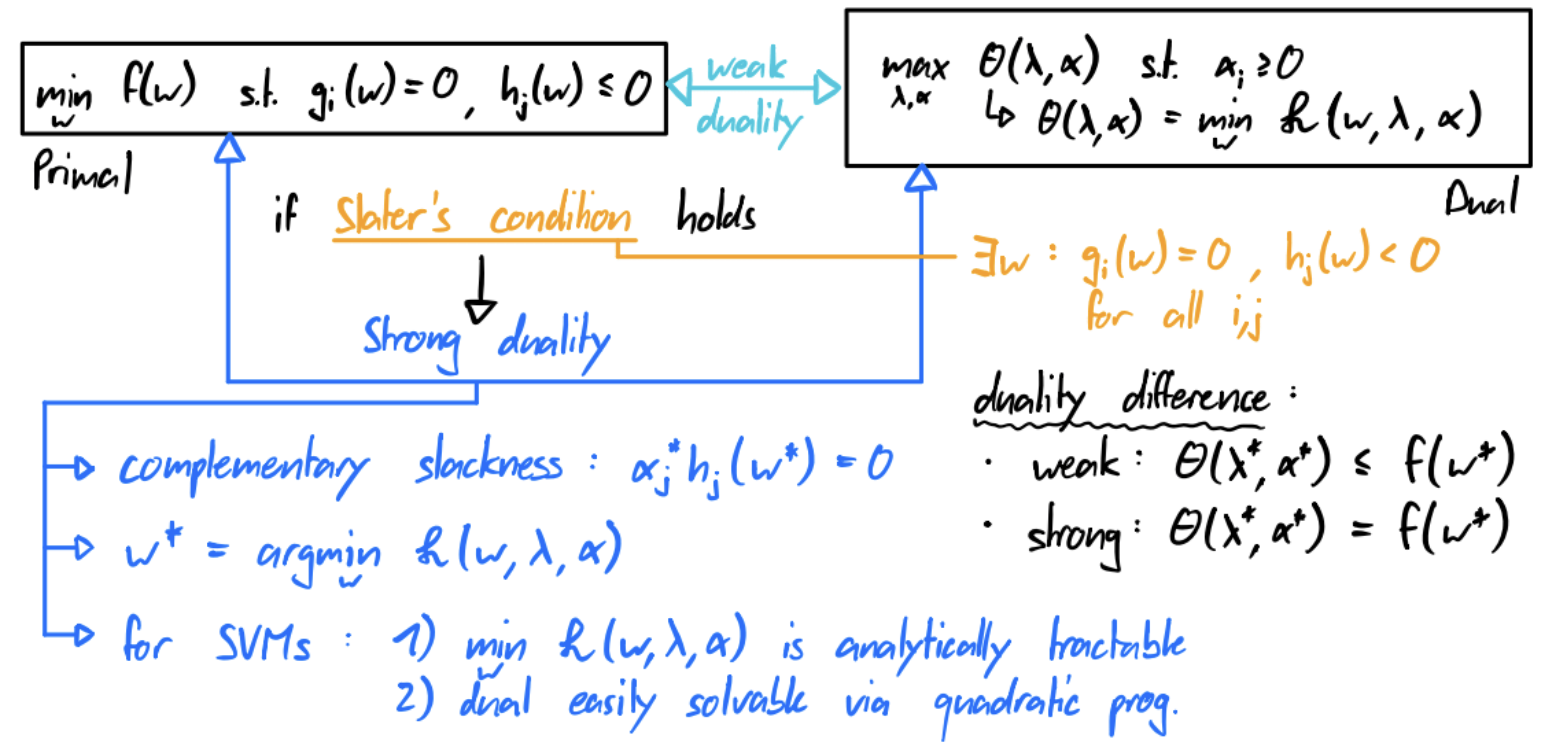
\includegraphics[width=7cm]{lagrangian multipliers.png}

\subsection*{SVMs}
\textbf{Primal Problem}: 
    {\scriptsize ($C \rightarrow \infty$: Hard Margin)}\\
    {\footnotesize $\min_w \frac{1}{2} w^Tw + C \sum_{i=1}^n \xi_i$ s.t. $y_i(w^T x_i +w_0) \geq 1-\xi_i, \, \xi_i \geq 0$ }\\
\textbf{Dual Problem}:
    $\mathcal{L}(w, w_0, \lambda, \alpha) = \frac{1}{2} w^\top w + \sum_{i \leq n} \alpha_i (1 - y_i(w^\top x_i + w_0))$, $\alpha_i \geq 0$ \\
    {\footnotesize $\Rightarrow \mathcal{L}(w^*, w_0^*, \lambda, \alpha) = - \frac{1}{2} \sum_{i,j} \alpha_i \alpha_j y_i y_j x_i^\top x_j + \sum_i \alpha_i$} \\
    $\Rightarrow \max_\alpha \alpha_i - \frac{1}{2} \sum_{i,j} \alpha_i \alpha_j \y_i y_j x_i^\top x_j$ s.t $\alpha_i \geq 0$, $\sum_i \alpha_i y_i = 0$ \\
    	%$\mathcal{L}(w,w_0,\xi,\alpha,\beta) = \frac{1}{2}w^Tw + C\sum_{i=1}^n\xi_i - \sum_{i=1}^{n}\beta_i\xi_i \\
        %\tab\tab\tab-\sum_{i=1}^{n} \alpha_i(z_i(w^T\phi(y_i) + w_0) -1+\xi_i)\\
		%\max_\alpha L(a) = \sum_{i=1}^n\alpha_i - \frac{1}{2} \sum_{i,j=1}^n z_i z_j 
		%\alpha_i \alpha_j \phi(y_i, y_j)\\
		%s.t. \, \sum_{j=1}^n z_j \alpha_j = 0 \, \wedge C \geq \alpha_i \geq 0 $\\
    $\Rightarrow$ optimal hyperplane:  $w^* = \sum_{i=1}^n \alpha_i^* y_i \phi(x_i)$, \\
    $w_0^* = -\frac{1}{2} (w^*^\top x^+ + w^*^\top x^-$ 
%    $w_0^* = \frac{1}{n_s} \sum_{i \in S}(z_n - \sum_{j \in S} \alpha_j z_j \phi(y_i,y_j))\\
%    		\stackrel{\text{\tiny linear}}{=} -\frac{1}{2}(min_{i:z_i=1} w^{*T}y_i + max_{i:z_i=-1} w^{*T}y_i)$\\
%Only for support vectors:\mbox{} $\alpha_i^* > 0$\\
%Prediction:\mbox{} 
%	$z(y)=sign(\sum_{i=1}^n \alpha_i z_i \phi(y,y_i) + w_0) \\
%        \stackrel{\text{\tiny linear}}{=} sign(w^{*T}x+w_0)$\\
%Homog. Coordinates:\mbox{}  condition $\sum_{j=1}^n z_j \alpha_j = 0$ falls away.

\subsection*{Kernelized SVMs}
\textbf{Training}: $\min_{\alpha} \sum_{i\leqn} \alpha_i - \frac{1}{2} \sum_{i,j \leq n} \alpha_i \alpha_j y_i y_j k(x_i, x_j)$ s.t. $\alpha \geq 0$, $\sum_i \alpha_i y_i = 0$ \\
\textbf{Classify}: $y = sign(\sum_{i \leq n} \alpha_i y_i k(x_i, x))$

\subsection*{Multiclass SVMs}
$\min_{w, \xi\geq 0} \frac{1}{2} w^T w + C \sum_i \xi_i$ s.t. \\
$(w_{y_i}^\top x_i + w_{y_i, 0}) - \max_{y \neq y_i} (w_y^\top x_i + w_{y,0}) \geq 1 - \xi_i$
%s.t. $\forall y_i \in Y:( w_{z_i}^T y_i) - max_{z \not = z_i} (w_z^T y_i) \geq 1-\xi_i$

\subsection*{Structured SVMs}
$\min_{w, \xi} \frac{1}{2} w^\top w + C \sum_i \xi$ s.t. \\
$w^\top \psi(x_i, y_i) - \max_{y \neq y_i} (w^\top \psi(x_i, y) \geq 1 - \xi$

% \subsection*{How to find $a^T$?}
% $a = \{w_0,w\}$ used along $\widetilde{x} = \{1,x\}$

% Gradient Descent: $a(k+1) = a(k) - \eta(k) \nabla J(a(k))$

% Newton method: 2nd order Taylor to get $\eta_{opt} = H^{-1}$ with $H=\frac{\partial^2 J}{\partial a_i \partial a_j}$

% $J$ is the cost matrix, popular choice is


% \subsection*{Perceptron Algorithm}
% Stochastic Gradient + Perceptron loss\\

% \emph{Theorem:} If $D$ is linearly seperable $\Rightarrow$ Perceptron will obtain a linear seperator.

% \subsection*{Support Vector Machine}
% Try to maximize a 'band' around the seperator.\\

% \subsection*{Matrix-Vector Gradient}
% %multiply transposed matrix to the same side as its occurance w.r.t. derivate variable: $\beta \in \mathbb{R}^d$
% $\nabla_\beta ( ||y-X\beta||_2^2 + \lambda ||\beta||_2^2 ) = 2X^T (y-X\beta) + 2\lambda \beta$\\

% \subsection*{Hinge loss}
% loss for support vector machine.\\
% $l_{SVM}(w,x_i,y_i) = \max \{0,1-y_iw^Tx_i\} + \lambda ||w||_2^2$\\
% derivation:\\
% $\frac{\partial}{\partial w_k} l_{SVM}(w,y_i,x_i) = \left \{
% \begin{array}{lr}
% 0 \text{ , if } 1-y_iw^Tx_i < 0 \\
% -y_ix_{i,k} + 2\lambda w_k \text{ , otherwise}
% \end{array} \right.	$

% \subsection*{Sparse L1-SVM}
% $\underset{w}{\operatorname{argmin}} \sum \limits_{i=1}^n \max (0, 1-y_i w^T x_i) + \lambda ||w||_1$

	% -*- root: Main.tex -*-
\section{Ensemble method}

\textbf{Classif. Trees}: shallow $\rightarrow$ bias$\uparrow$, variance$\downarrow$, deep $\rightarrow$ bias$\downarrow$, variance$\uparrow$

\textbf{Bagging}: train \textit{simple} classifier on different data sets $\Rightarrow$ variances$\downarrow$, covar.$\downarrow$ and biases$\downarrow$ \\
$\hat{b}(x) = \left\{ \begin{array}{ll} \frac{1}{M}\sum_{t \leq M} b^{(t)}(x) & \mathrm{regression} \\ \mathrm{vote}\{ b^{(1)}, \cdots, b^{(M)} \} & \mathrm{classification}   \end{array} \right.$

\textbf{Boosting}: adaptive combination of poor learners with sufficient diversity $\Rightarrow$ var.$\downarrow$, biases$\downarrow$

\begin{comment}
\subsection*{Random Forest}
for b=1:B do:\\
draw a bootstrap sample $D_b$\\
repeat until node size<$n_{min}$:\\
1. select $m$ features from $p$ features\\
2. pick the best variable and split-point\\
3. Split the node accordingly\\
return the forest $\{\hat{c}_b(x)\}_{b=1}^B$
\end{comment}

%Boosting: Train weak learners sequentially on all data, but reweight misclassifed samples higher, Bias $\downarrow$
\subsection*{Adaboost}
Initialize weights $w_i = 1/n$, for $b = 1,...,B$ do: \\
1. Fit classifier $c_b(x)$ with weights $w_i$ \\
2. Compute error $\epsilon_b = \sum_i w_i^{(b)} \mathbbm{1}_{[c_b(x_i) \not = y_i]} / \sum_i w_i^{(b)}$\\
3. Compute coeff. $\alpha_b = log(\frac{1-\epsilon_b}{\epsilon_b})$\\
4. Update weights $w_i = w_i \exp(\alpha_b \mathbbm{1}_{[y_i \not = c_b(x_i)]})$
Return $\hat{c}_B(x) = \text{sign} \left ( \sum_{b=1}^B \alpha_b c_b(x) \right )$\\

\textbf{Loss}: Exponential loss function\\
\textbf{Model}: Additive logistic regression\\
Bayesian approach (assumes posteriors),
Newton-like updates (Gradient Descent)

%\newpage

%\subsection*{Bagging}
%\textbf{for} $b=1$ to $B$ \textbf{do}:\\
%1. $Z^{*b}=$ b-th bootstrap sample from Z\\
%2. Construct classifier $c_b$ based on $Z^{*b}$\\
%\textbf{return} ensemble class. $\hat{c}_B(x)=sgn(\sum_{i=1}^{B} c_i(x))$\\
%\textbf{Works}: Covariance small (different subset for training), Variance small (similar behaviour of weak learners), biases weakly affected.\\
%\textbf{Bag. aggr. pred.}: $h_B(x)=E_{D'\sim D}[h_{D'}(x)]$\\
%\textbf{Ideal aggr. pred.}: $h_A(x)=E_{D\sim P(x,y)}[h_D(x)]$\\
%$E_D[L(y,h_D(x))]=E_D[(y-h_D(x))^2]=E_D[y^2]-2E_D[y\cdot h_D(x)]+E_D[h_D(x)^2]=y^2-2y\cdot E_D[h_D(x)]+E_D[h_D(x)^2]\geq y^2-2y\cdot E_D[h_D(x)]+E_D[h_D(x)]^2=y^2-2y\cdot h_A(x)+h_A(x)^2=(y-h_A(x))^2=L(y,h_A(x))$\\
%\textbf{Bias$\downarrow$\&Var.$\downarrow$}: Use complex decision tree (bias$\downarrow$), ensemble mult. decision trees (var$\downarrow$)

	\section{Deep Learning}

\textbf{Robbins-Monro}: finds root of reg. function \\
$x_{n+1} = x_n - \alpha_n y_n = x_n - \alpha_n f(x_n)$, where \\
(1) $\lim_{n\rightarrow \infty} \alpha_n = 0$ {\tiny conv.}, (2) $\sum_{n=1}^\infty \alpha_n = \infty$ {\tiny slow},\\
(3) $\sum_{n=1}^\infty \alpha_n^2 < \infty$ {\tiny bounded var.}

\textbf{Kiefer-Wolfowitz}: finds min. of reg. function \\
$x_{n+1} = x_n - \alpha_n \frac{f(x_n + c_n) - f(x_n - c_n)}{2 c_n}$, where \\
(1), (2) from before, (3) $\lim_{n\rightarrow \infty} c_n = 0$, \\
(4) $\sum_{n=1}^\infty (\frac{\alpha_n}{c_n})^2 < \infty$

\subsection*{Gradient Descent}
Taylor: {\footnotesize $f(x_n + \triangle x) = f(x_n) + \nabla f(x_n)^\top \triangle x + \frac{1}{2} \triangle x^\top H \triangle x$} \\
$\Rightarrow$ optimal step: $x_{n+1} = x_n - \frac{\nabla f^\top \nabla f}{\nabla f^\top H \nabla f} \cdot \nabla f$

\textbf{Newton's Rule}: $x_{n+1} = x_n - H^{-1} \nabla f(x_n)$

\textbf{Momentum}: $y_{n+1} = x_n + \beta \cdot (x_n - x_{n-1})$, \\$x_{n+1} = y_{n+1} - \alpha_n \nabla f(y_{n+1})$

\subsection*{Backpropagation}
For each unit $j$ on the output layer:\\
- Compute error signal: $\delta_j = \ell_j'(f_j)$\\
- For each unit $i$ on layer $L$: $\frac{\partial}{\partial w_{j,i}} = \delta_j v_i$

For each unit $j$ on hidden layer $l=\{L-1,..,1\}$:\\
- Error signal: $\delta_j = \phi'(z_j) \sum_{i\in Layer_{l+1}} w_{i,j}\delta_i$\\
- For each unit $i$ on layer $l-1$: $\frac{\partial}{\partial w_{j,i}} = \delta_j v_i$

\subsection*{Autoencoder}
learns binary encoding or its inverse {\tiny discrete}\\
learns compressed, distr. repres. (|lin. hidden units| < |in/out units| $\rightarrow PCA$) {\tiny continous}

\textbf{Variational Autoencoder (VAE)}: \\
Decoder: $p_\Theta (x) = \int p_\Theta (z) p_\Theta (x|z) dz$,\\  Encoder $q_\phi (z|x)$ approx. $p_\Theta (x|z)$ \\
$\log p_\Theta(x_i) = \mathbb{E}_z [\log p_\Theta(x_i|z)] - \mathbb{E}_z [\log \frac{q_\phi (z|x_i)}{p_\Theta (z)}] + \mathbb{E}_z [\log \frac{q_\phi(z|x_i)}{p_\Theta(z|x_i)}] = \mathcal{L}(x_i, \Theta, \phi) + \mathbb{E}_z [\log \frac{q_\phi(z|x_i)}{p_\Theta(z|x_i)}]$ \\
\textbf{ELBO}: $log p_\Theta (x_i) \geq \mathcal{L}(x_i, \Theta, \phi)$

	\section{Nonparametric Bayesian Learning}
$Dir(x|\alpha) = \frac{1}{B(\alpha)} \prod_{k=1}^n x_k^{a_k - 1}$, $B(\alpha) = \frac{\prod_{k=1}^n \Gamma(\alpha_k)}{\Gamma(\sum_{k=1}^n \alpha_k)}$ \\
$\mathbb{E}[1] = \sum_{i=1}^N \frac{\alpha}{\alpha + i} \sim(\alpha log(N))$ \\
de Finetti: $p(X_1, ..., X_n) {=} \int (\prod_{i=1}^n p(x_i|G))dP(G)$ \\
\[ p(z_i=k|\bm{z}_{-i},\bm{x},\alpha,\bm{\mu}) = \begin{cases}
      \frac{N_{k,-i}}{\alpha + N - 1} p(x_i|\bm{x}_{-i,k},\bm{\mu}) \;\exists k \\
      \frac{\alpha}{\alpha + N - 1} p(x_i|\bm{\mu}) \;\text{otherwise}
   \end{cases}
\]
DP generative model: \\
\begin{inparaitem}[\color{red}\textbullet]
\item Centers of the clusters: $\mu_k \sim \mathcal{N}(\mu_0, \sigma_0)$ \\
\item Prob.s of clusters: $\rho = (\rho_1, \rho_2) \sim  GEM(\alpha)$ \\
\item Assignments to clusters: $z_i \sim Categorical(\rho)$ \\
\item Coordinates of data points: $\mathcal{N}(\mu_{z_i}, \sigma)$
\end{inparaitem}
	% -- PAC LEARNING
\section{PAC Learning}
Empirical error: $\hat{\mathcal{R}}_n(c) = \tfrac{1}{n}\sum_{i=1}^n \mathbb{I}_{\{c(x_i)\neq y\}}$ \\
Expected error: $\mathcal{R}(c) = P\{c(x)\neq y\}$ \\
ERM: $\hat{c}_n^* = \argmin_{c\in\mathcal{C}} \hat{\mathcal{R}}_n(c)$ \\
opt: $c^* \in \min_{c\in\mathcal{C}} \mathcal{R}(c)$, $|\mathcal{C}|$ finite \\
Generalization error: $\mathcal{R}(\hat{c}_n^*) = P\{ \hat{c}_n^*(x)\neq y \}$ \\
VC ineq.: $\mathcal{R}(\hat{c}_n^*) - \inf\limits_{c\in\mathcal{C}}\mathcal{R}(c) \leq 2\sup\limits_{c\in\mathcal{C}}|\hat{\mathcal{R}}_n(c) - \mathcal{R}(c)|$ \\ 
$P\{ \mathcal{R}(\hat{c}_n^*) - \mathcal{R}(c^*) > \epsilon \} \leq P\{ \sup\limits_{c\in\mathcal{C}}|\hat{\mathcal{R}}_n(c) - \mathcal{R}(c)| > \frac{\epsilon}{2} \} \\
\leq 2|\mathcal{C}| exp(-2n\epsilon ^2 /4) \leq 8s(\mathcal{A},n)exp(-n\epsilon ^{2} /32)$ and $s(\mathcal{A},n) \leq n^{\mathcal{V_{\mathcal{A}}}}$ \\
Markov ineq: $P\{X\geq\epsilon\} \leq \tfrac{\mathbb{E}[X]}{\epsilon}$ (for nonneg. X) \\
Boole's inequality: $P(\bigcup_i A_i) \leq \sum_i P(A_i)$ \\
Hoeffding's lemma: $\mathbb{E}[e^{sX}] \leq exp(\tfrac{1}{8}s^2(b-a)^2)$ where $\mathbb{E}[X]=0$, $P(X\in[a,b])=1$ \\
Hoeffding's: $P\{S_n {-} \mathbb{E}[S_n] {\geq} t\} {\leq} exp({-} \frac{2t^2}{\sum_i (b_i - a_i)^2})$ \\
Normalized: $P\{\widetilde{S}_n {-} \mathbb{E}[\widetilde{S}_n] {\geq} \epsilon\} {\leq} exp({-} \frac{2n^2 \epsilon ^2}{\sum_i (b_i {-} a_i)^2})$ \\
{\small Error bound: $P\{ \sup\limits_{c\in\mathcal{C}}|\hat{\mathcal{R}}_n(c) - \mathcal{R}(c)| > \epsilon \} \leq 2|\mathcal{C}| exp(-2n\epsilon ^2)$} \\
The $\mathcal{VC}$ dimension of a model $f$ is the maximum number of points that can be arranged so that $f$ shatters them.
    % -*- root: Main.tex -*-
\section{Good To Know Stuff}
\subsection*{Numerical Estimating Methods}
Actual Risk: $\mathcal{R}(f) := \E_{x,y}[l(y-f(x))]$ \\
Empiricial Risk: $\hat{\mathcal{R}}(f) = \frac{1}{n}\sum_i l(y_i - f(x_i))$\\
Generalization Error: $G(f) = |\hat{\mathcal{R}}(f) - \mathcal{R}(f)|$

\subsection*{K-fold cross validation}
$\hat{f}^{-\nu} \in \argmin_f \frac{1}{|Z^{-\nu}|} \sum_{i \in Z^{-\nu}} (y_i - f(x_i))^2$\\
$\hat{\mathcal{R}}^{cv} = \frac{1}{n} \sum_i(y_i - \hat{f}^{-\kappa(i)}(x_i))^2$, $k(i)$ is fold $i^{th}$ fold \\
Problem: systematic tendency to underfit.

\subsection*{Leave-one-out}
unbiased, high variance \\
$\hat{f}^{-i} \in \argmin_f \frac{1}{n-1} \sum_{j:j \neq i} L(y_i,f(x_i))$ \\
$\hat{\mathcal{R}}^{LOOCV} = \frac{1}{n} \sum_i L(y_i, \hat{f}^{-i}(x_i))$

\subsection*{Bootstrapping}
Resampling with replacement from data $D$ to produce $B$ boostrap datasets $D^{*b}$.  $S(D)$ is expected generalization error of prediction model trained on $D$. Var: $\sigma ^2(S) = \frac{1}{B-1}\sum_{b=1}^B(S(D^{*b})-\bar{S})^2$ with mean: $\hat{R}_{boot}(f)=\bar{S}=\frac{1}{B}\sum_{b=1}^B(\frac{1}{N}\sum_{i=1}^NL(y_i,\hat{f}_{D^{*b}}(x_i)))$ with $\hat{f}_{D^{*b}}(x_i)$ being the prediction model. $\hat{R}_{boot}^{LOO}(f) = \frac{1}{N}\sum_{i=1}^N\frac{1}{|C^{-i}|}\sum_{b\in C^{-i}}L(y_i,\hat{f}_{D^{*b}}(x_i))$ where $C^{-i}$ denotes the set of bootstrap sets not containing data point $i$. Note: $L$ can be $I_{\{c(x_i)\not =y_i\}}$.
$\hat{R}_{boot}$ is optimistic. Hence use: $\hat{R}^{.0632}=0.368\hat{R}_{boot}+0.632\hat{R}_{boot}^{(LOO)}$. \\
Prob. not to appear in set: $(1-\frac{1}{n})^n = \frac{1}{e}$ for $n \rightarrow \infty$

\subsection*{Information Criteria}
$BIC = ln(n)k - 2ln(\hat{L})$, $AIC = 2k - 2ln(\hat{L})$\\
$TIC = 2trace[I_1(\theta_k)J_1^{-1}(\theta_k)] - 2ln(\hat{L})$, 
where k: num. params, n: num. data points, likelihood: $\hat{L}=p(X|\theta_k,M)$  

\subsection*{Loss-Functions}
True class: $y \in \{-1,1\}$, pred. $x \in [-1,1]$\\
Cross-entropy (log loss): ($y'=\tfrac{(1+y)}{2}$ and $x'=\tfrac{(1+x)}{2}$) $L(y',x') {=} -[y'log(x') {+} (1-y')log(1-x')]$ \\
Hinge Loss: $L(y,x) = max(0, 1-yx)$ \\
Perceptron Loss: $L(y,x) = max(0, -yx)$ \\
Logistic loss: $L(y,x) = log(1 + exp(-yx))$ \\
Square loss: $L(y,x) = \tfrac{1}{2}(1-yx)^2$ \\
Exponential loss: $L(y,x) = exp(-yx)$ \\
Binomial deviance: $L(y,x) = 1 + exp(-2yx)$ \\
0/1 Loss: $L(y,x) = \mathbb{I}\{sign(x)\neq y\}$

\subsection*{Perceptron} 
Gradient descent: $a(k+1) = a(k) - \eta(k)\nabla J(a(k))$ \\
$J(a)\approx J(a(k))+\nabla J^T(a-a(k)) + \tfrac{1}{2}(a-a(k))^T H (a-a(k))$, $H{=}\frac{\partial^2 J}{\partial a_i \partial a_j}$ \\
$2^{nd}$ order algorithm: $\eta_{opt} = \frac{\norm{\nabla J}^2}{\nabla J^T H \nabla J}$ \\
Newton's rule: $a(k+1){=}a(k){-}H^{{-}1}\nabla J$\\
Perceptron criteria: $J_p(a)=\sum_{\widetilde{x}\in\widetilde{\mathcal{X}}^{mc}} (-a^T \widetilde{x})$ \\
Perceptron rule: $a(k+1)=a(k)+\eta(k)\sum_{\widetilde{x}\in\widetilde{\mathcal{X}}^{mc}} \widetilde{x}$ \\
Perceptron convergence:$\left \| a(k+1)- \alpha \hat a \right \|^{2} = \left \| a(k)- \alpha \hat a \right \|^{2}  + 2(a(k)- \alpha \hat a)^{T} \tilde x^{k} + \left \| \tilde x^{k} \right \|^{2} \leq \left \| a(k)- \alpha \hat a \right \|^{2} -2\alpha \gamma + \beta ^{2}$
where $\beta^{2} = max_{i}  \left \| \tilde x_{i \in \tilde X^{mc} } \right \| ^{2}$ and $\gamma = min_{i \in \tilde X^{mc} } (\hat a^{T} \tilde x_{i}) > 0 $ for $\alpha= \beta^{2} / \gamma$  then $k_{0}= \alpha^{2}\left \|\hat a \right \|^{2} / \beta^{2}=  \beta^{2}\left \|\hat a \right \|^{2} / \gamma^{2}$

\subsection*{Gaussian Mixtures}
	Estimate $\hat{\theta} = \{\mu_1,...,\mu_k, \Sigma_1,...,\Sigma_k\}$ that maximize the likelihood of sample feature vectors $\mathcal{X} = \{x_1,..., x_n \}$: \\
	$p(\mathcal{X} | \pi_i, ..., \pi_k, \theta_1, ..., \theta_k) = \prod_{x \in \mathcal{X}} \sum_{c\leq k}  \pi_c p(x|\theta_c)$\\
	Log-Likelihood: $L(\mathcal{X} | \pi, \theta) = \sum_{x\in \mathcal{X}}
	 \log \sum_{c \leq k} \pi_c p(x|\theta_c)$
	
\subsection*{Expectation Maximization}
$L(\X,M|\theta) = \sum_{x \in \X} \sum_{c=1}^k M_{xc} \log(\pi_c P(x|\theta_c)$ \\
$Q(\theta; \theta^{(j)}) = \E_{M}[L(\X,M|\theta)| \X, \theta^{(j)}]$, M latent variable

$M_{xc} = 1$ if cluster $c$ has generated $x$, else $M_{xc} = 0$
$\\ \E_M[M_{xc}|\X, \theta^{(j)}] = P(M_{xc}=1) = P(c | x, \theta^{(j)}) = 
\frac{P(x|c,\theta^{(j)}) P(c|\theta^{(j)})}{P(x|\theta^{(j)})}
= \frac{\pi_c P(x|c,\theta^{(j)})}{\sum_{c=1}^K \pi_c P(x|c,\theta^{(j)})} 
=: \gamma_{xc}$
\begin{algorithmic}[1]
	\While{not converged}
	\State E-Step:
		\tab Compute $\gamma_{xc}$ for all $x, c$
		\tab Compute $m_c := \sum_x \gamma_{xc}$ for all $c$
	\State M-Step: max $Q(\theta; \theta^{(j)}) \hspace{5mm} s.t. \sum_c \pi_c = 1$
    	\vspace{-3mm}
    	\addtolength{\jot}{-3mm}
		\begin{align*}
			\mu_c^{(j+1)} &= \tfrac{\sum_{x \in \mathcal{X}} \gamma_{xc} x}{m_c} \hskip 15pt  
			\pi_c^{(j+1)} = \tfrac{1}{|\mathcal{X}|} m_c \\
			\Sigma_c^{(j+1)} &= \tfrac{\sum_{x \in \mathcal{X}} \gamma_{xc}(x-\mu_c)(x-\mu_c)^T}
				{m_c} 
		\end{align*}
        \vspace{-6mm}
	\EndWhile
\end{algorithmic}

\textbf{Lagrangian with fixed $\gamma_{xc}$} \mbox{}\\
$L = \sum_x \sum_c \gamma_{xc} \log(\pi_c P(x|c,\theta_c)) - 
\lambda(\sum_c \pi_c - 1)$\\
For GMM: $P(x|c,\theta^{(j)}) = \mathcal{N}(x | \mu_c, \Sigma_c)$

\subsection*{Generative Methods}

\textbf{Naive Bayes} \\
All features independent.\\
$
P(y|x) = \frac{1}{Z} P(y) P(x|y), Z = \sum_{y} P(y) P(x|y) \\
y = \argmax_{y'} P(y'|x) = \argmax_{y'} \hat{P}(y') \prod_{i=1}^{d} \hat{P}(x_i|y')
$ \\
\textbf{Discriminant Function}\\
$
f(x) = \log(\frac{P(y=1|x)}{P(y==1|x)}), y=sign(f(x))
$

\subsection*{Neural Network: Learning features}
Parameterize the feature maps and optimize over the parameters:\\
$w^* = \underset{w, \Theta}{\operatorname{argmin}} \sum_{i=1}^n l(y_i, \sum_{j=1}^m w_j \Phi(x_i, \Theta_j))$

\textbf{Reformulating the perceptron} \\
Ansatz: $w=\sum_{j=1}^n \alpha_j y_j x_j$\\
$\min \limits_{w\in\mathbb{R}^d} \sum_{i=1}^n \max [0, -y_i w^T x_i]$\\
$= \min \limits_{\alpha_{1:n}} \sum_{i=1}^n \max [0,-y_i  ( \sum_{j=1}^n \alpha_j y_j x_j  )^T x_i ]$\\
$= \min \limits_{\alpha_{1:n}} \sum_{i=1}^n \max  [0,- \sum_{j=1}^n \alpha_j y_i y_j x_i^T x_j ]$
        
\textbf{Kernelized Perceptron} \\
1. Initialize $\alpha_1 = ... = \alpha_n = 0$\\
2. For t do \\
Pick data $(x_i,y_i) \in_{u.a.r} D$\\
Predict $\hat{y} = sign(\sum_{j=1}^n \alpha_j y_j k(x_j,x_i))$\\
If $\hat{y} \not = y_i$ set $\alpha_i = \alpha_i + \eta_t$
	
% -*- root: Main.tex -*-





	
%		\subsection*{Regularization}
%	The error term $L$ and the regularization $C$ with regularization parameter $\lambda$: $\min \limits_w L(w) + \lambda C(w)$\\
%	L1-regularization for number of features \\
%	L2-regularization for the length of $w$
	
%	\subsection*{Convex}
%	$\text{g(x) is convex}$\\
%	$\Leftrightarrow x_1,x_2 \in \mathbb{R}, \lambda \in [0,1]:$\\
%	$g(\lambda x_1) + (1-\lambda x_2) \leq \lambda g(x_1) + (1-\lambda) g(x_2)$
%	$ \Leftrightarrow g''(x) > 0$

%	\subsection*{Parametric to nonparametric linear regression}
%	Ansatz: $w=\sum_i \alpha_i x$\\
%	Parametric: $w^* = \underset{w}{\operatorname{argmin}} \sum_i (*Tx_i-y_i)^2 + \lambda ||w||_2^2$\\
%	$= \underset{\alpha_{1:n}}{\operatorname{argmin}} \sum \limits_{i=1}^n (\sum \limits_{j=1}^n \alpha_j x_j^T x_i - y_i)^2 + \lambda \sum \limits_i \sum \limits_j \alpha_i \alpha_j (x_i^T x_j)$\\
%	$= \underset{\alpha_{1:n}}{\operatorname{argmin}} \sum \limits_{i=1}^n (\alpha^T K_i - y_i)^2 + \lambda \alpha^T K \alpha$\\
%	$= \underset{\alpha}{\operatorname{argmin}} ||\alpha^T K -y||_2^2 + \lambda \alpha^T K \alpha$\\
%	Closed form: $\alpha^* = (K+\lambda I)^{-1} y$\\
%	Prediction: $y^*= w^{*^T} x = \sum \limits_{i=1}^n \alpha_i ^* k(x_i,x)$

\end{multicols*}
\end{document}